\chapter{Analyse}
\label{chap:analyse}
la reproduction des résultats de Mme Yerly est la première étape du projet.
Elle est importante car c'est mon premier travail sur une application concrète d'un problème de \acrlong{ml} et j'ai besoin de ces bases pour la suite du projet.
Pour cette étape je vais m'inspirer du rapport\cite{IL_SVM_report} de Mme Yerly et je vais reproduire les résultats à l'aide \acrlong{sklearn}.


\section{Lecture des données}
Pour récolter les donées, j'ai plusieurs sources mais la source officielles est un fichier Excel\cite{SVM_data} qui contient un dataset d'entraînement, un de test et des candidats fournis par ChemTech.
Les autres sources de données sont des fichiers txt générer par Mme Yerly à partir du fichier Excel.
La particularité de ces fichiers c'est que les features et les targets ont été normalisées avec l'agorithme MinMax dans un script \acrshort{r}.

Pour lire les données, j'ai utilisé la librairie \acrfull{pandas} pour les fichiers Excel et txt.
\begin{lstlisting}[language=Python]
import pandas as pd


def build_set(df, x_start, x_size, y_start, y_size):
    m = df.to_numpy()
    x = m[:, x_start:x_start + x_size]
    y = m[:, y_start:y_start + y_size]
    return x, y.ravel()


def import_from_excel(s_name):
    # Import data
    frame = pd.read_excel('ressources/SVM_data.xlsx',
                            sheet_name=s_name)
    frame.drop(0, axis=0, inplace=True)  # Remove line with image
    return build_set(frame, 2, 99, 101, 1)


def import_from_txt(f_name):
    frame = pd.read_csv('ressources/' + f_name, sep=":",
                        header=None)
    return build_set(frame, 1, 99, 0, 1)
\end{lstlisting}
La méthode \texttt{build\_set} prend en paramètre un dataframe \acrshort{pandas} et les indices de début et de fin des features et des targets.

Pour utiliser ces méthodes, il suffit de prendre exemple sur le code suivant pour les données d'Excel:
\begin{lstlisting}[language=Python]
X_train, y_train = import_from_excel('Training set')
X_test, y_test = import_from_excel('Testing set')
\end{lstlisting}
ou de cette façon pour les données des fichiers txt:
\begin{lstlisting}[language=Python]
X_train, y_train = import_from_txt('training_set_sklearn.txt')
X_test, y_test = import_from_txt('test_set_sklearn.txt')
\end{lstlisting}
Ces deux méthodes retournent les 99 features et la target dans deux tableaux numpy de taille 600 pour le training set et de 168 pour le test set.


\section{Préparation des données}
Comme le but est d'utiliser les données d'Excel, il faut trouver un moyen de les normaliser pour obtenir d'autant bon résultat que Mme Yerly.
Pour cela, j'ai utilisé la méthode \texttt{MinMaxScaler} de \acrlong{sklearn} qui permet de normaliser les données entre 0 et 1.
\begin{lstlisting}[language=Python]
def normalize(train, test):
    scaler = preprocessing.MinMaxScaler()
    train_norm = scaler.fit_transform(train)
    test_norm = scaler.transform(test)
    return train_norm, test_norm, scaler
\end{lstlisting}
Cette méthode prend en paramètre les données d'entraînement et de test et retourne les données normalisées et le scaler utilisé pour normaliser les données.
Le scaler est mis en forme sur le minimum et maximum des données d'entraînement et sera utilisé pour dénormaliser les données calculées par le modèle.


\section{Entraînement du modèle}
Dans le rapport\cite{IL_SVM_report} de Mme Yerly, c'est la librairie LIBSVM qui a été utilisée pour entraîner le modèle.
Pour reproduire les résultats, il est conseillé d'utiliser la librarire \acrlong{sklearn} qui est une librairie de machine learning qui contient des implémentations de plusieurs algorithmes de \acrlong{ml}.
L'avantage c'est que nous pouvons rapidement modifier les paramètres mais surout l'algorithme pour voir si les résultats sont meilleurs.
De plus, \acrlong{sklearn} utilise la librairie LIBSVM pour entraîner les modèles de type \acrshort{svm}.

Cependant, tout modèle utilise des paramètres qui modifient le comportement de l'algorithme et ces paramètres ne s'exprime pas de la même façon entre les deux librairies.
\begin{center}
    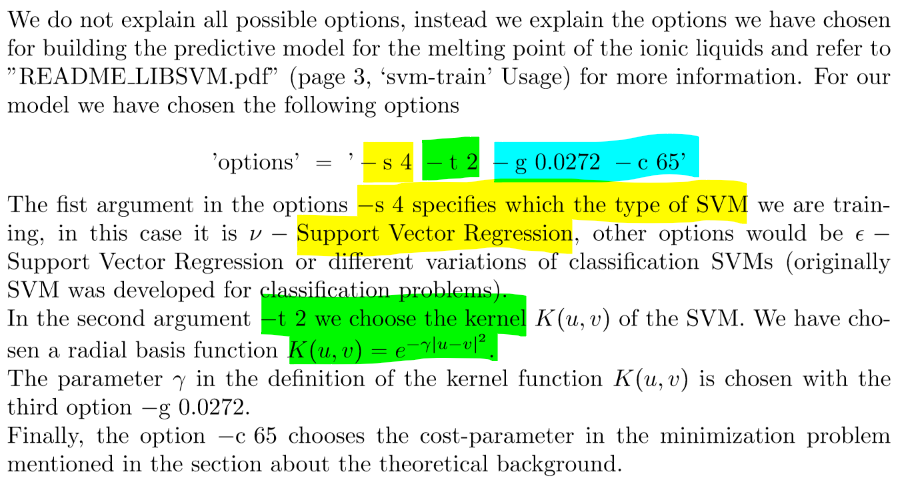
\includegraphics[width=130mm]{img/report-parameter.png}
    \captionof{figure}{Explication des paramètres du modèle}
\end{center}
Pour être encore plus précis, le paramètre \texttt{-s 4} correspond à l'algorithme \texttt{NuSVR}.

\begin{center}
    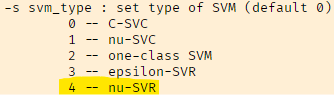
\includegraphics[width=70mm]{img/libsvm-parameter.png}
    \captionof{figure}{Algorithme \acrshort{svm} d'après la documentation de LIBSVM\cite{libsvm_doc}}
\end{center}

Cependant, l'algorithme \texttt{NuSVR} peut être utilisé avec différents types de noyaux.
L'argument \texttt{-t} permet de choisir ce kernel:
\begin{center}
    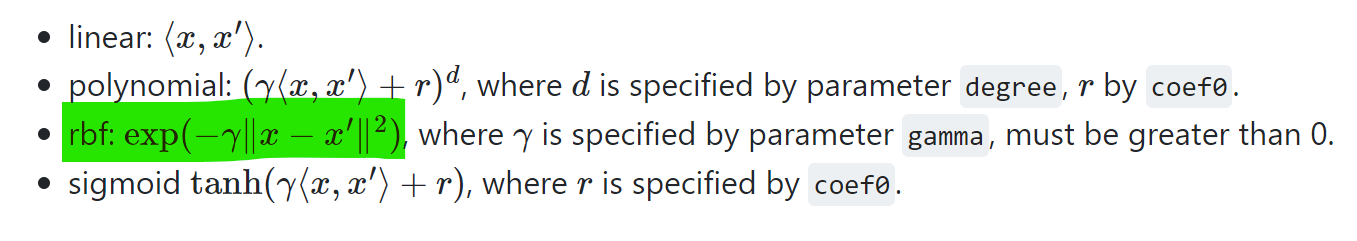
\includegraphics[width=130mm]{img/kernel-parameter.png}
    \captionof{figure}{Types de noyaux d'après la documentation de \acrlong{sklearn}\cite{scikit-learn}}
\end{center}

Pour finir, \texttt{-g} et \texttt{-c} peuvent être directement utilisé comme tel dans \acrlong{sklearn}.

Avec toutes les informations précédentes, j'ai pu créer le modèle avec les paramètres suivants:
\begin{center}
    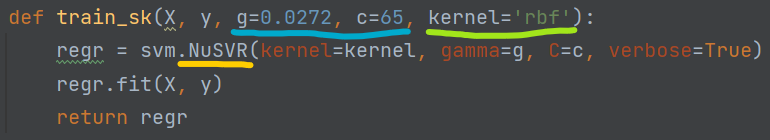
\includegraphics[width=130mm]{img/my-parameter.png}
    \captionof{figure}{Paramètres du modèle}
\end{center}


\section{Résultats}
Afin de comparer les résultats, je me base sur les indicateurs $R^2$ et \acrfull{mse} qui sont ceux utilisés par Mme Yerly dans sont rapport\cite{IL_SVM_report}.
Pour les calculer, j'ai utilisé la méthode suivante:

\begin{lstlisting}[language=Python]
def compute_result(regr,
                   X_train,
                   y_train,
                   X_test,
                   y_test,
                   y_scaler=None):
    predicted_test = regr.predict(X_test)
    predicted_train = regr.predict(X_train)

    R2_training = regr.score(X_train, y_train)
    R2_testing = regr.score(X_test, y_test)

    if not y_scaler is None:
        y_train = y_scaler.inverse_transform(
            y_train.reshape(-1, 1))
        predicted_train = y_scaler.inverse_transform(
            predicted_train.reshape(-1, 1))
        y_test = y_scaler.inverse_transform(
            y_test.reshape(-1, 1))
        predicted_test = y_scaler.inverse_transform(
            predicted_test.reshape(-1, 1))

    MSE_training = metrics.mean_squared_error(
        y_train,
        predicted_train)
    MSE_testing = metrics.mean_squared_error(
        y_test,
        predicted_test)

    print_result(MSE_training,
                 MSE_testing,
                 R2_training,
                 R2_testing)


def print_result(MSE_training,
                 MSE_testing,
                 R2_training,
                 R2_testing):
    print("\n\t\t\t\tResult")
    print("MSE training:\t" + str(MSE_training))
    print("MSE testing:\t" + str(MSE_testing))
    print("R^2 training:\t" + str(R2_training))
    print("R^2 testing:\t" + str(R2_testing))
\end{lstlisting}

Le code suivant, utilisent toutes les méthodes précédentes pour entraîner le modèle et calculer les résultats et les comparer avec ceux de Mme Yerly.
\begin{lstlisting}[language=Python]
X_train, y_train = import_from_excel('Training set')
X_test, y_test = import_from_excel('Testing set')
X_train_norm, X_test_norm, _ = normalize(X_train, X_test)
y_train_norm, y_test_norm, y_scaler = normalize(
                                        y_train.reshape(-1, 1),
                                        y_test.reshape(-1, 1))
y_train_norm = y_train_norm.ravel()
y_test_norm = y_test_norm.ravel()

regr = train_sk(X_train_norm, y_train_norm)

compute_result( regr,
                X_train_norm,
                y_train_norm,
                X_test_norm,
                y_test_norm,
                y_scaler)
\end{lstlisting}


\subsection{Synthèse des résultats}
Les résultats sont les suivants:
\begin{table}[h]
    \centering
    \begin{tabular}{l|l|l|}
    \cline{2-3}
                                                    & \textbf{Training set} & \textbf{Test set} \\ \hline
    \multicolumn{1}{|l|}{\textbf{$R^2$ goal}}          & 87\%                  & 82.5\%            \\ \hline
    \multicolumn{1}{|l|}{\textbf{$R^2$ reproduction}}  & 86.9\%                & 81.8\%            \\ \hline
    \multicolumn{1}{|l|}{\textbf{MSE goal}}         & 386.85                & 515.47            \\ \hline
    \multicolumn{1}{|l|}{\textbf{MSE reproduction}} & 386.97                & 516.12            \\ \hline
    \end{tabular}
    \captionof{table}{Résultats}
\end{table}
Les résultats sont assez similaires pour considérer que la reproduction est réussie.


\subsubsection{Autres résultats}
Tester de reproduire les résultats avec d'autres paramètres.
